\subsection{Test setup}

Our program was written in C/C++ and compiled with Clang. All memory allocations were cache line boundary aligned. For parallelization we used C++11 cross-platform library \texttt{<thread>}.

All benchmarks were performed on a Linux desktop which has 16 GB ram and a Core i7 3770 CPU with the following specification:

\begin{itemize}
\item 4 * 3.4 GHz (Turbo Boost up to 3.9 GHz)
\item 4 * 32 KB L1 instruction cache
\item 4 * 32 KB L1 data cache (write back)
\item 4 * 256 KB L2 cache (write back)
\item Hyper-Threading
\item Shared 8 MB L3 cache (inclusive, write back)
\item 64 byte cache lines
\item The associativity for the cache levels are 8, 8 and 16 respectively
% http://www.ni.com/white-paper/11266/en#toc5
\end{itemize}

L2 cache faults and L3 cache faults were measured using Intel Performance Monitor Counter while branch mispredictions were measured using PAPI.

All tests were performed 5 times and the median was selected. The data in the matrices were randomly generated double precision floating points with
an uniform distribution. The range of the data was -1 to
1.

\subsection{Simple multiplication}

\subsubsection{Row-based layout}
Figure~\ref{fig:rnrnrn0} shows the measured running time and cache
faults encountered when running the naive matrix multiplier on
matrices with row layout.
\begin{figure}[h!]
  \centering
  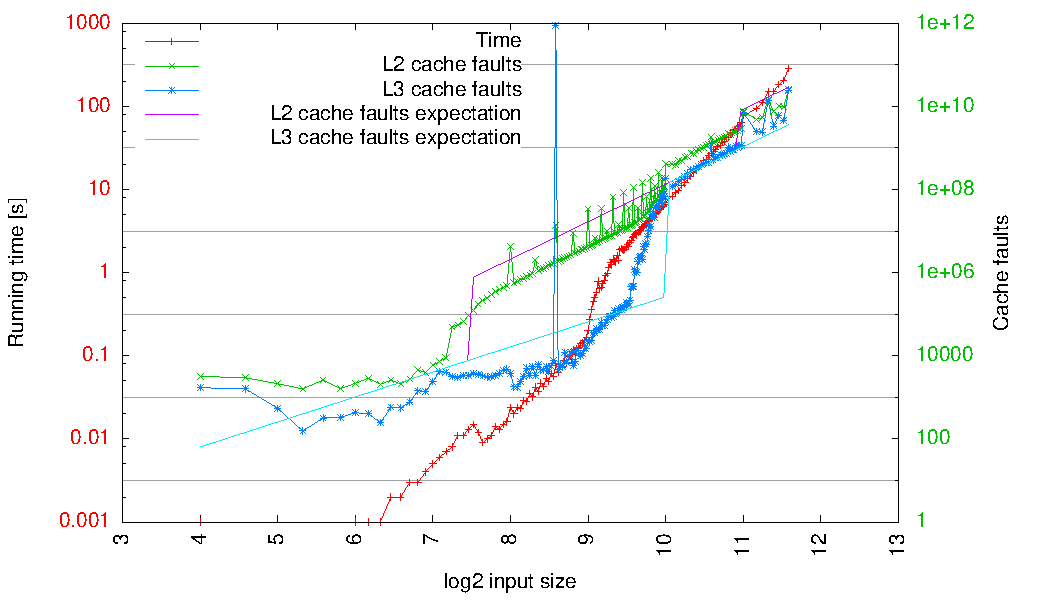
\includegraphics[width=\textwidth]{plots/rowrow.pdf}
  \caption{Running time and cache faults of naive matrix
    multiplication with all matrices using row layout.}
  \label{fig:rnrnrn0}
\end{figure}

From figure~\ref{rnrnrn0} it seems like we typically gets a bit fewer
cache faults than we expect\todo{Describe why?}. The jumps we expect
also seems to happen, although in the experiments, they seem to happen
a bit before we expect. This can be explained by that the cache also
contains some data which is not the matrices.

Figure~\ref{rnrnrn0} moreover shows a lot of spikes on the lines
indicating L2 and L3 cache faults. The L2 spikes is beginning around
$n = 256$ and the L3 spikes around $n = 1024$.

We strongly suspect that the cache layout due to the 8-way
associativity is to blame. When looking up in the L2 cache, the 36 bit
physical address of the i7 processor is split into three parts $addr =
(tag,index,offset)$. Since the cache line size is $64b$, $6$ bits
should be used to reference a byte in a cache line. Because the L2
cache is $256kb$, we find that the index size to be
\[
  \frac{256 \cdot 1024}{\underbrace{64}_{\text{Cache line size}} \cdot \underbrace{8}_{\text{Cache associativity}}}
    = 512 = 2^9.
\]
Hence, we should use $9$ bits to specify the index. The remaining
$36-6-9=21$ bits is used as tag. Notice that the tag is the most
significant part of the address.

Because the size of our matrices is always divisible by the cache line
size, it will always be the case that a new row in a matrix starts
with a new cache line. But this means that a cache line, and the
corresponding cache lines on the next row, always will be
$\frac{n}{B}$ cache lines apart. Therefore we are only able to utilize
$\ord(\frac{n}{B})$, cache lines in the L2 cache, where $\ord(\dot)$
denotes the order of the element in the additive group
$\mathbb{Z}_{2^9}$.

Figure~\ref{fig:rowrow_cachepeaks} illustrates the correlation between
these available cache lines in the cache (the green line), and the
cache misses divided by the expected number of cache misses (the red
line).

When comparing the interval from $[7.5; 9]$ with the interval $[9;
  10]$, the green line seems to dictate significant more peeks in the
$[9; 10]$ interval. This also makes sense, since the matrices in this
case are bigger, meaning that more columns of the $B$ matrix will be
loaded. Therefore we will overwrite the same available cache slots
more times (we can afford to do this 8 time, since we have an 8-way
cache). The plot on figure~\ref{fig:rowrow_cachepeaks} heavily suggest
that these peaks actually stems from the 8-way cache layout.  The
peaks on the line plotting the L3 cache faults, the peaks can be
described in a similar fashion.

\begin{figure}[h!]
  \centering
  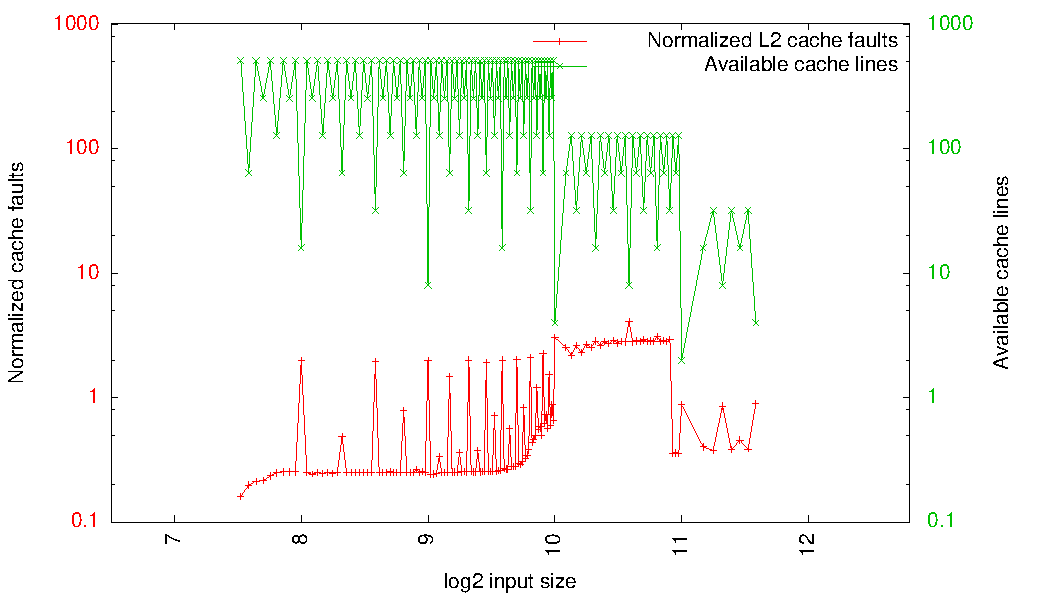
\includegraphics{plots/rowrow_cachepeaks}
  \caption{The number of available cache lines vs. the number of cache
    faults occurring in experiments.}
  \label{fig:rowrow_cachepeaks}
\end{figure}

It can be seen from figure~\ref{fig:rnrnrn0} that the running time
becomes a lot worse at $2^9 = 512$. At this points when we jump from
one row to another in the $B$ matrix, we jump a distance of $512 \cdot
8 = 4096$ bytes. This is the page size of the system, so we jump
exactly a page for every read. Moreover, the size of the second-level
TLB in the i7 processor can hold $512$ entries and uses a pseudo-LRU
replacement strategy, leading to a TLB miss every time we read a cell
in the $B$ matrix. This explains why we see the running time becomes
worse at this point.

\subsubsection{Row/column-based layout}
Next we performed experiments where we stored the $A$ matrix in row
form, the $B$ matrix in column form and saved the result in matrix $C$
in row form. From the algorithms section, we believe this to perform
better than the row-row naive multiplication.

\begin{figure}[h!]
  \centering
  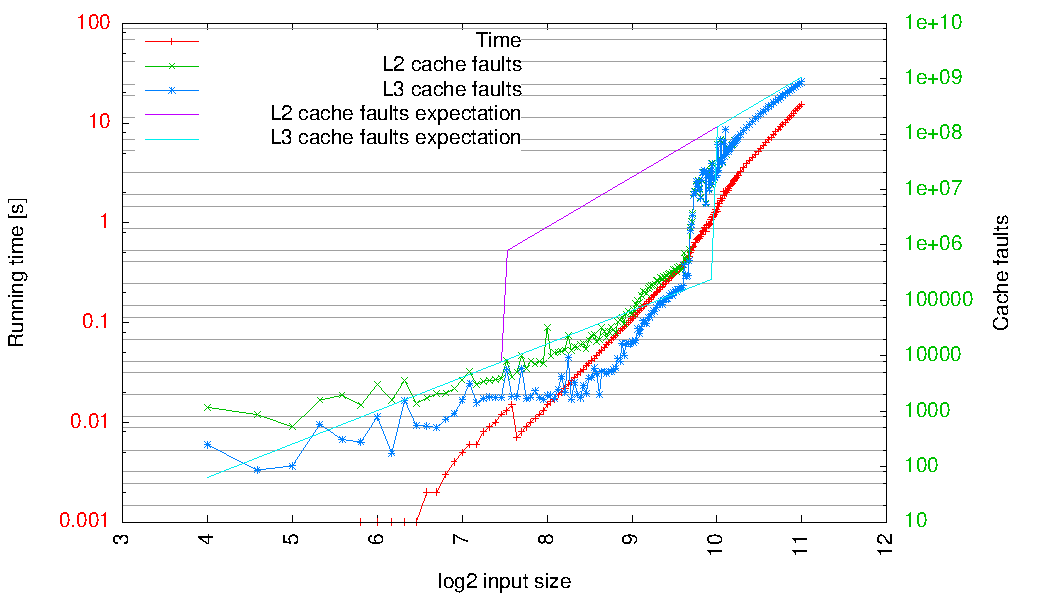
\includegraphics[width=\textwidth]{plots/rowcol}
  \caption{Running time and cache faults using naive matrix
    multiplication with row and column layout.}
  \label{fig:rowcol}
\end{figure}

One thing to notice in figure~\ref{fig:rowcol} is that the number of
L2 cache faults seems to follow the number of L3 cache faults. This
was not what we expected. As shown by the purple line at the plot, we
would expect the number of L2 cache faults to become significantly
worse at input size $n \approx 180$, when the $B$ matrix does not fit
the cache anymore.

In order to explain this behavior we have tried to disassemble the
program to verify that the compiler did not make any very clever
unexpected optimizations. This turned out not to be the case.

We then tried to make a simple model of the i7 L2 cache, where we
simulated the 8-way cache layout\footnote{The simulation was based on
  the description of the i7 L2 cache described in Computer
  Architecture: A Quantitative Approach, 5th edition. Cite this
  probably! We also tried the simulation on the row-row layout, this
  corresponded quite nicely with the real world, hinting some sanity
  of the simulation.}. In this experiment, we also tried to fill out
the matrix one row at a time, but start from the right end half of the
times. This should give us a better cache
performance. Figure~\ref{fig:rowcolsimulation} shows the result of
this simulation compared to the actual number of cache faults.
\begin{figure}[h!]
  \centering
  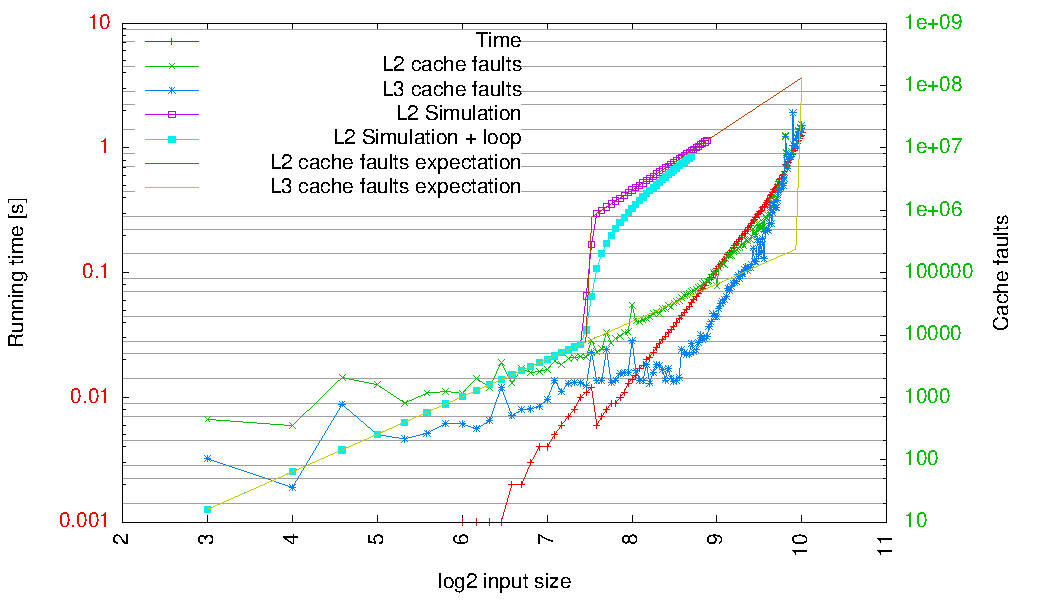
\includegraphics[width=\textwidth]{plots/rowcol_simulation}
  \caption{Simulated cache performance vs. the actual cache performance.}
  \label{fig:rowcol_simulation}
\end{figure}

As figure~\ref{fig:rowcol_simulation} illustrates, the simulated cache
performance very nicely follows our expectations. Changing the
for-loop so that we start filling out from the right half of the times
helps a bit on the cache performance, but can not explain the
real-life L2 cache performance.

This hints that there is some hardware in the CPU, that in this case
is doing a really good job to minimize the L2 cache faults. We tried
to run the experiments on a smaller computer with an i3-550 processor
where we disabled the hardware- and adjacent cache line
prefetchers. This test, however, turned out inconclusive\footnote{We
  got some very strange looking results from the test. The test was
  performed running a live linux distribution booted from an USB
  storage stick, but the stick broke during the next restart of the
  machine. Hence, if our code made some call to the operating system
  not loaded into memory, our results could be heavily influenced by
  malfunctioning hardware. Therefore we do not have a lot of
  confidence in the results.}.

Figure~\ref{fig:rowcol_vs_rowrow} is comparing the row-column results
to the row-row results. This plot shows the row-row results divided by
the row-column results. From the algorithms section, we will expect
the improvement factor to be greater than $1$.
\begin{figure}[h!]
  \centering
  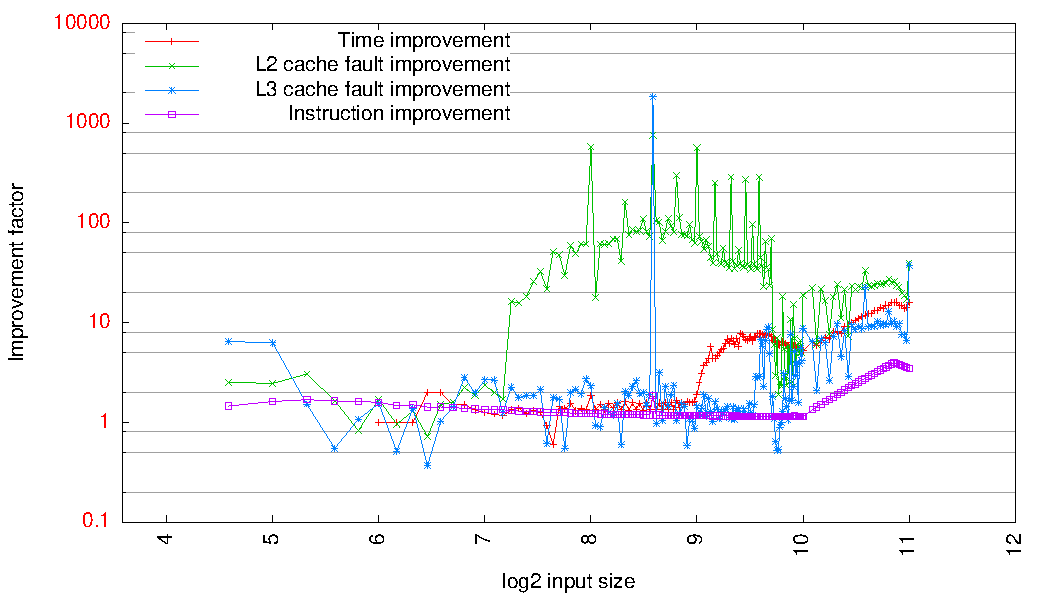
\includegraphics[width=\textwidth]{plots/rowcol_vs_rowrow}
  \caption{Relative performance of row-row vs. row-col
    layout. Improvement factor indicates how many times row-col
    performs better than row-row.}
  \label{fig:rowcol_vs_rowrow}
\end{figure}

It can be seen that the row-column version begins to perform a lot
better at $n \approx 2^9$, which is where the row-row layout begin to
experience lots of TLB misses.

The plots shows an improved cache performance and running time of the
row-column layout. However, the plot also shows that the row-row
layout begins to perform more instructions when the size of the
matrices exceeds $2^{10} = 1024$. We suspect this could be because the
operating system needed to perform some additional work to manage the
virtual memory / paging.

\subsection{Recursive multiplication}

Figure \ref{fig:recursive_layout_performance} shows the performance of the two layouts with the best base case size of each. As can be seen on the figure, the best performing layout of the recursive algorithm is the tiled layout. And, as expected, the recursive algorithm outperforms the naive row/column algorithm.

\subsubsection{Layouts}

The tiled layout is better at utilizing the cache shown in figure \ref{fig:recursive_layout_cachefaults}. Furthermore, the Z-curved layout uses more instructions. Recall that, the Z-curve offsets are precomputed but the extra level of indirection and offset calculations increases the number of instructions.

The best Z-curve base size is much smaller than the best tiled layout base case size. By having a small base case we use the recursion for more levels which means that we do not spend as many instructions on looking up offsets in the precomputed table as we do with larger base cases. However, when the base case gets very small then the instructions used on invoking a method and the conditional statements and jumps from loops gets significant.

%\ref{fig:zrzrzr0}

%\begin{figure}[h!]
%  \centering
%  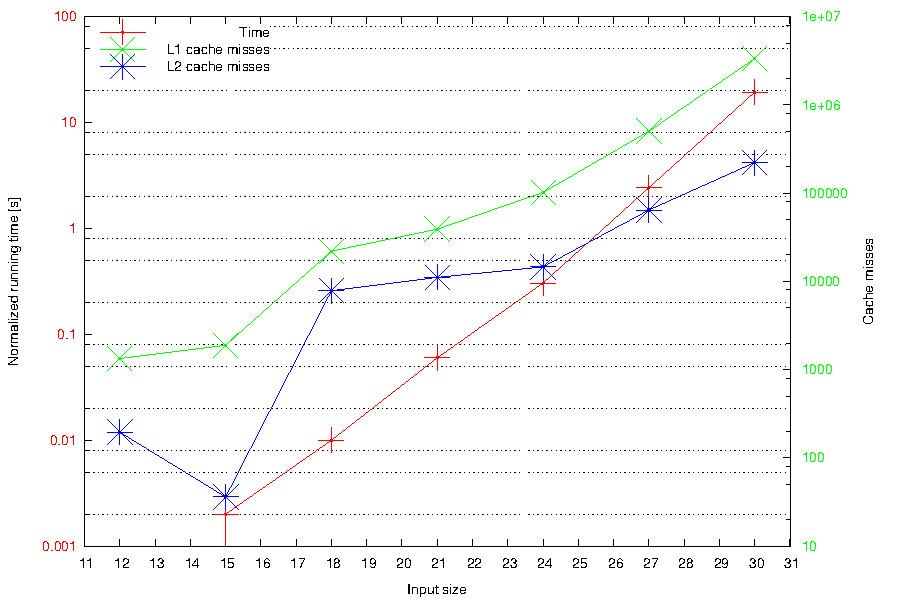
\includegraphics[width=\textwidth]{zrzrzr0.pdf}
%  \label{fig:zrzrzr0}
%\end{figure}

%\subsubsection{Tiled layout}

%\begin{figure}[h!]
%  \centering
%  \includegraphics[width=\textwidth]{"../project2/gnuplots/recursive_base_cases"}
%  \caption{Performance of the recursive algorithm with different base case sizes.}
%  \label{fig:recursive_base_cases}
%\end{figure}

\begin{figure}[h!]
  \centering
  \includegraphics[width=\textwidth]{"../project2/gnuplots/recursive_performance"}
  \caption{Performance comparison between different layouts and the naive row/column algorithm.}
  \label{fig:recursive_layout_performance}
\end{figure}

\begin{figure}[h!]
  \centering
  \includegraphics[width=\textwidth]{"../project2/gnuplots/recursive_cache"}
  \label{fig:recursive_layout_cachefaults}
  \caption{Cache faults for each layout.}
\end{figure}

\begin{figure}[h!]
  \centering
  \includegraphics[width=\textwidth]{"../project2/gnuplots/recursive_instructions"}
  \label{fig:recursive_layout_instructions}
  \caption{Number of instructions for the recursive and naive algorithm.}
\end{figure}

\subsection{Strassen}

%\begin{figure}[h!]
%  \centering
%  \includegraphics[width=\textwidth]{"../project2/gnuplots/strassen_base_cases"}
%  \caption{Performance of Strassen with different base case sizes.}
%  \label{fig:recursive_base_cases}
%\end{figure}

\begin{figure}[h!]
  \centering
  \includegraphics[width=\textwidth]{"../project2/gnuplots/recursive_vs_strassen_performance"}
  \caption{Performance of the best recursive and best Strassen.}
  \label{fig:recursive_vs_strassen_performance}
\end{figure}

Figure \ref{fig:recursive_vs_strassen_performance} shows that Strassen performs better than the tiled recursive algorithm for all the matrix sizes we have tested. However, figure \ref{fig:recursive_vs_strassen_cache} does not give the expected number of cache misses. The increased number of cache faults might be due to large constants in the big Theta notation for all the additions, subtractions etc.

\begin{figure}[h!]
  \centering
  \includegraphics[width=\textwidth]{"../project2/gnuplots/recursive_vs_strassen_cache"}
  \caption{Cache misses of the recursive and Strassen.}
  \label{fig:recursive_vs_strassen_cache}
\end{figure}

%\begin{figure}[h!]
%  \centering
%  \includegraphics[width=\textwidth]{"../project2/plots/4096/row-tiled8x8 recursive-8(tiled-bc)_column-tiled-8x8 recursive-8(generic-bc)_row-tiled8x8 recursive-8(tiled-bc)_0"}
%  \caption{Recursive}
%\end{figure}



%\begin{figure}[h!]
%  \centering
%  \includegraphics[width=\textwidth]{"../project2/plots/4096/z-curve-tiled strassen-32(32-fixed-tiled-bc)_z-curve-tiled strassen-32(32-fixed-tiled-bc)_z-curve-tiled strassen-32(32-fixed-tiled-bc)_0"}
%  \caption{Strassen}
%\end{figure}

\subsection{SIMD instructions}

We experienced a substantial performance speedup when SIMD instructions were used (figure \ref{fig:simd}). An increase is in line with our expectations. The amount of cache faults stayed the same in the tests as expected while the cache hits was greatly reduced.

As can be seen, the speedup using SIMD instructions for the recursive algorithm is higher than for Strassen. This is likely due to a larger number of cache faults for Strassen. This makes the proportion of time used on fetching data higher.

\begin{figure}[h!]
  \centering
  \includegraphics[width=\textwidth]{"../project2/gnuplots/simd_performance"}
  \label{fig:simd}
  \caption{Speedup using SIMD instructions.}
\end{figure}

\subsection{Parallelization}

\begin{figure}[h!]
  \centering
  \missingfigure{Lav graf over performance af Strassen, rekursiv og row/column naiv. 8 core m/ht Og sammenlign med single cpu}
  \label{fig:parallel_performance}
  \caption{Performance of parallelized algorithms.}
\end{figure}

We have analyzed the theoretical speedup using non-linear regression and Amdahl's law. The percentage of parallelized code in the iterative and recursive algorithms are 98\% while our implementation of Strassen have 89\% parallelized code. This could be improved by parallelizing the last additions and the code for combining submatrices. The projected speedup is shown in figure \ref{fig:amdahl}. The speedup is when SIMD instructions are included.

\begin{figure}[h!]
  \centering
  \includegraphics[width=\textwidth]{"../project2/gnuplots/amdahl"}
  \label{fig:amdahl}
  \caption{Speedup projection using Amdahl's law.}
\end{figure}